\documentclass{jsarticle}
\usepackage{graphicx,listings}
\lstset{language={C},%
  basicstyle=\footnotesize,%
  commentstyle=\textit,%
  classoffset=1,%
  keywordstyle=\bfseries,%
  frame=tRBl,framesep=5pt,%
  showstringspaces=false,%
  numbers=left,stepnumber=1,numberstyle=\footnotesize%
}%


\title{情報実験第三 1.C}

\author{情報工学科15\_03602 柿沼 建太郎 \\ 情報工学科 15\_10588 中田 光}
\date{\today}
\begin{document}
\maketitle

\section*{各課題担当者}
各課題と担当者を表として以下に示す。
\begin{table}[h]
\begin{tabular}{|l|c|c|} \hline
課題番号/名前 & 柿沼 & 中田 \\ \hline \hline
素数プログラム &  & $\circ$ \\ \hline
test\_calc1 & $\circ$ & \\ \hline
test\_io2 & $\circ$ & $$ \\ \hline
\end{tabular}
\end{table}

\newpage

\section*{FPGA実装レポート}

\subsection*{課題1. 素数プログラムにN以下の素数を全て出力する機能を追加し、FPGAで動作検証する}
担当:中田\\

\subsubsection*{概要}
以前作成した素数プログラムをもとに作成した。アルゴリズムは課題1.Aと同様で与えられたNに対し
それ以下の全ての自然数で除算を行うことで判定している。\\
入力Nは16進の4桁とし、出力はN以下の素数を空白ごとに10進数で出力している。Nを入力しENTERを押すと結果が出力される。\\
\\
※FFFFは実行時間が膨大になると考えられたので途中で中断した実行結果である。


\subsubsection*{実行結果}


\begin{figure}[htbp]
 \begin{minipage}{0.5\hsize}
  \begin{center}
  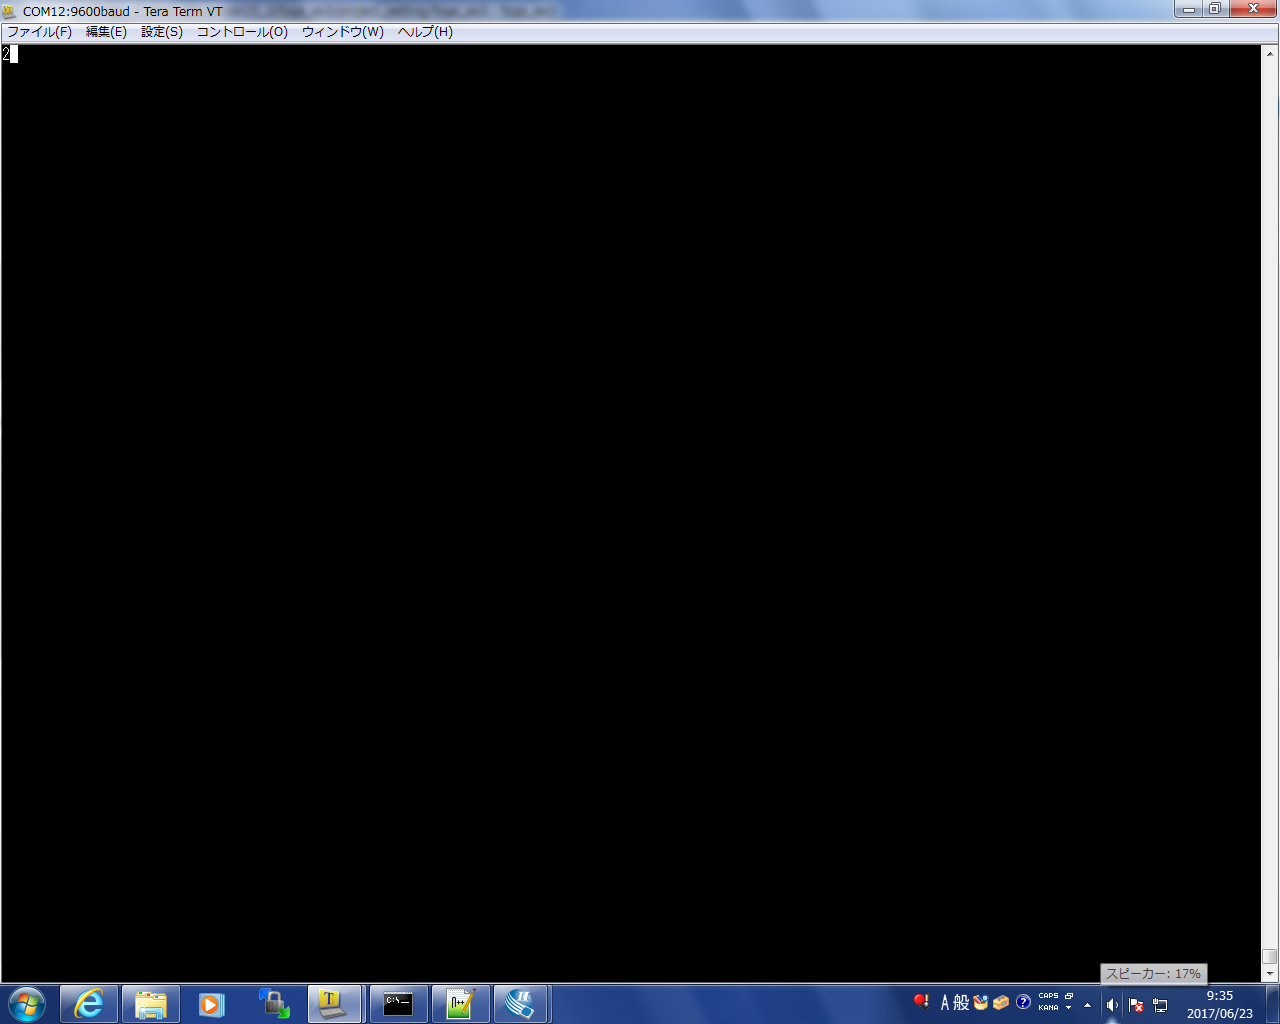
\includegraphics[width=8cm,bb=0 0 1280 1024]{2out.png}
  \end{center}
  \caption{"2"}
 \end{minipage}
 \begin{minipage}{0.5\hsize}
  \begin{center}
   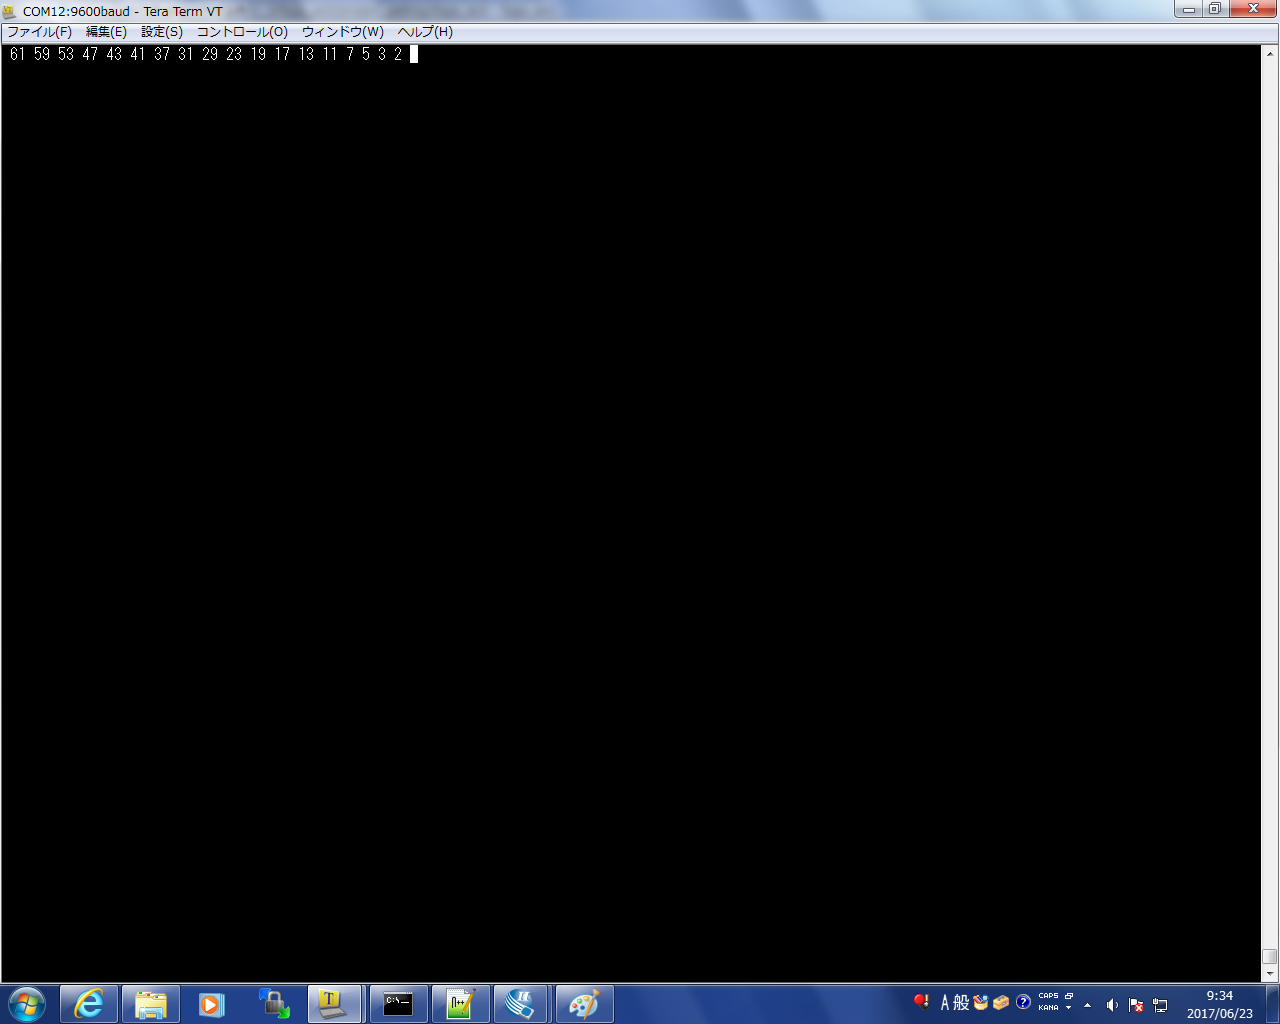
\includegraphics[width=8cm,bb=0 0 1280 1024]{40out.png}
  \end{center}
  \caption{"40"}
 \end{minipage}
\end{figure}

\begin{figure}[htbp]
 \begin{minipage}{0.5\hsize}
  \begin{center}
  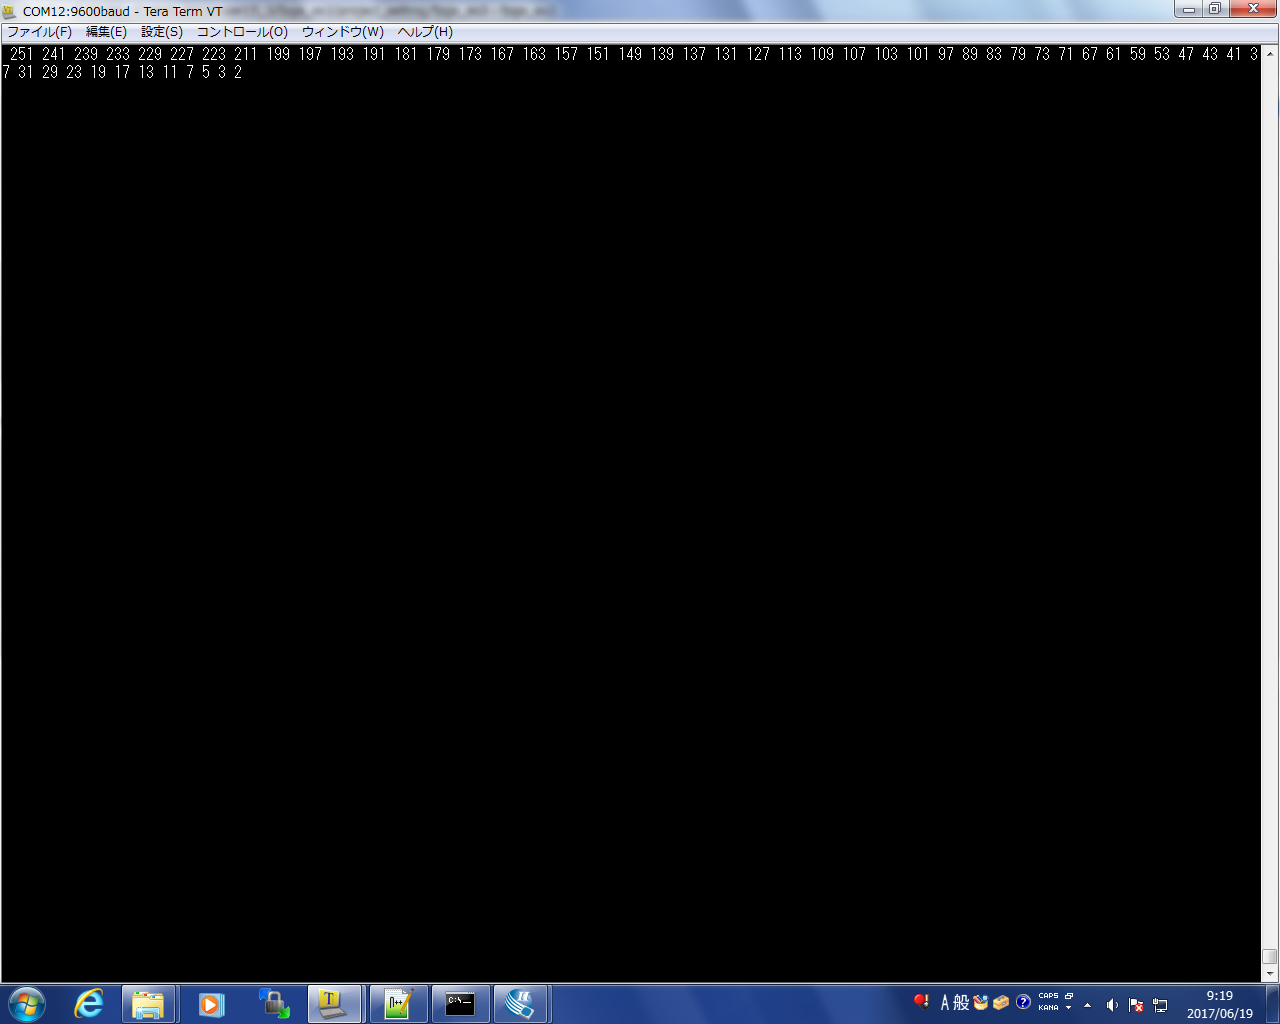
\includegraphics[width=8cm,bb=0 0 1280 1024]{FFout.png}
  \end{center}
  \caption{"FF"}
 \end{minipage}
 \begin{minipage}{0.5\hsize}
  \begin{center}
   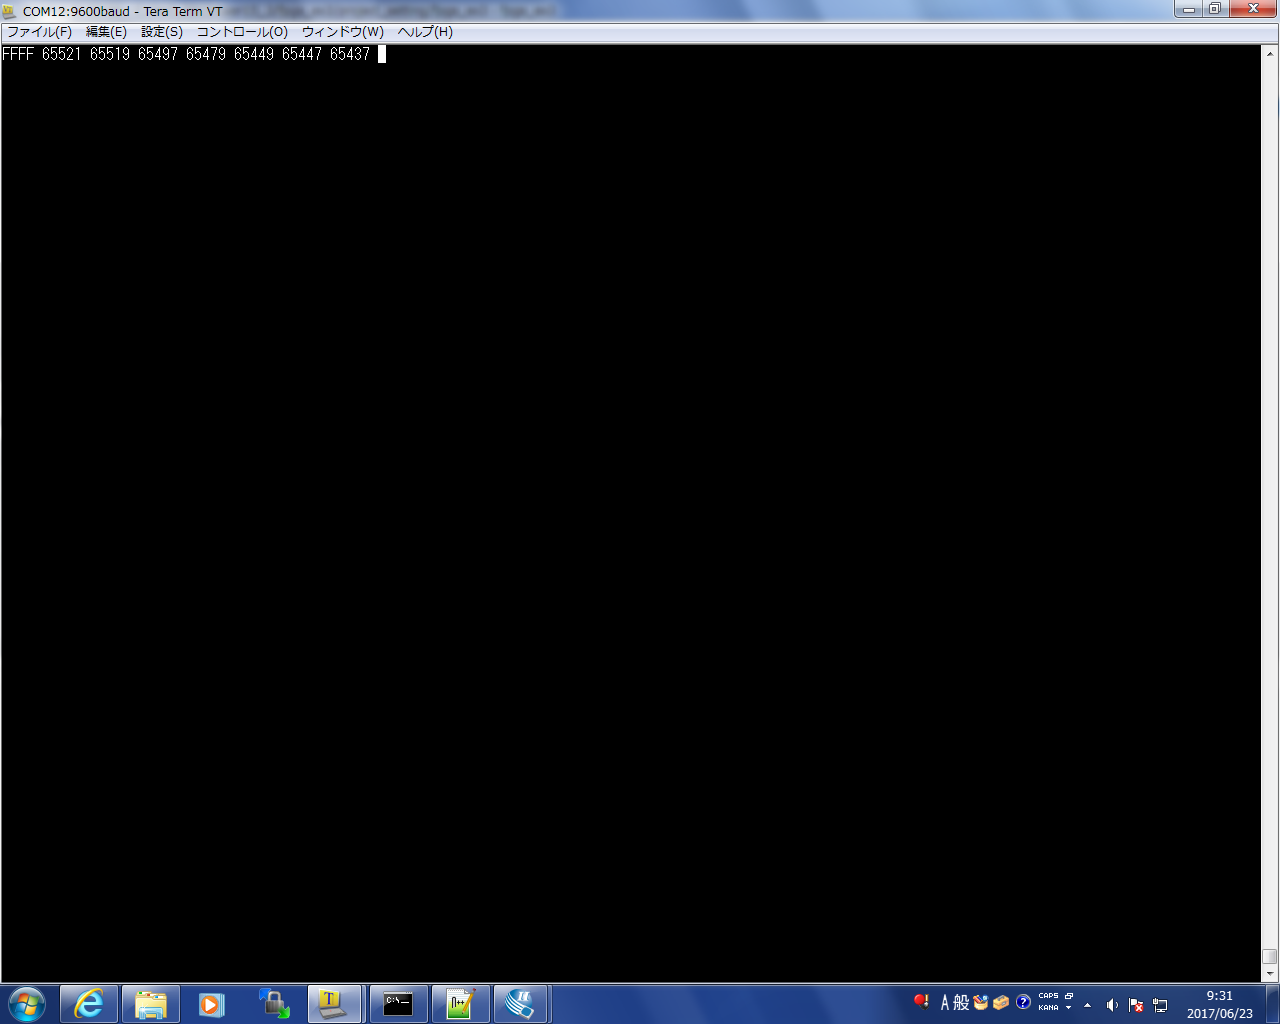
\includegraphics[width=8cm,bb=0 0 1280 1024]{FFFFinout.png}
  \end{center}
  \caption{"FFFF"}
 \end{minipage}
\end{figure}

\newpage

\subsubsection*{ソースコード}

\lstinputlisting[caption=素数プログラム]{./report1_4_nakata_verilog3.asm}

\subsubsection*{感想}
素数プログラムを改良するのにあたって、入出力機能の追加や16進から10進の変換は課題1.Aで作成したプログラムや
test\_io1を組み合わせることで作成できたため、割と早い段階で作ることができた。
だが、FGOが1になり書き込み可能になるのを待たずに書き込みを行おうとしてしまい、シミュレーションではうまく動いていたが、
FPGAでは出力が正しくされず、原因に気づくのに時間がかかってしまった。
FPGAとシミュレーションで動きが違うため、シミュレーションで動くものがFPGAで動かないことが多々あったので
そこが改善されて欲しいと感じた。

\newpage


\subsection*{課題2.test\_calc1の計算結果を7セグメントディスプレイに表示するように改良し、FPGAで動作検証する}
担当:柿沼\\
\subsubsection*{概要}
ex3の命令セットに空きがあることがわかっていたため、新しい命令「SEG」を追加し、それを用いて7セグメントディスプレイに計算結果を表示することとした。
与えられたVerilogコードでは実行状態では7セグメントディスプレイに現在のPCの値が16進数表記で表示されることになっていたが、命令拡張をするにあたり、実行状態では新たに作ったレジスタ「seg」の中身を常に16進数表示で表示することとした。
SEG命令は呼び出されると、その時点でのACの値をsegレジスタに転送する命令とした。
以上の命令拡張及び仕様変更を加え、test\_calc1.asmの値を表示する箇所付近にSEG命令を挿入することで計算結果を表示した。

\subsubsection*{実行結果}

\begin{figure}[htbp]
 \begin{minipage}{0.5\hsize}
  \begin{center}
  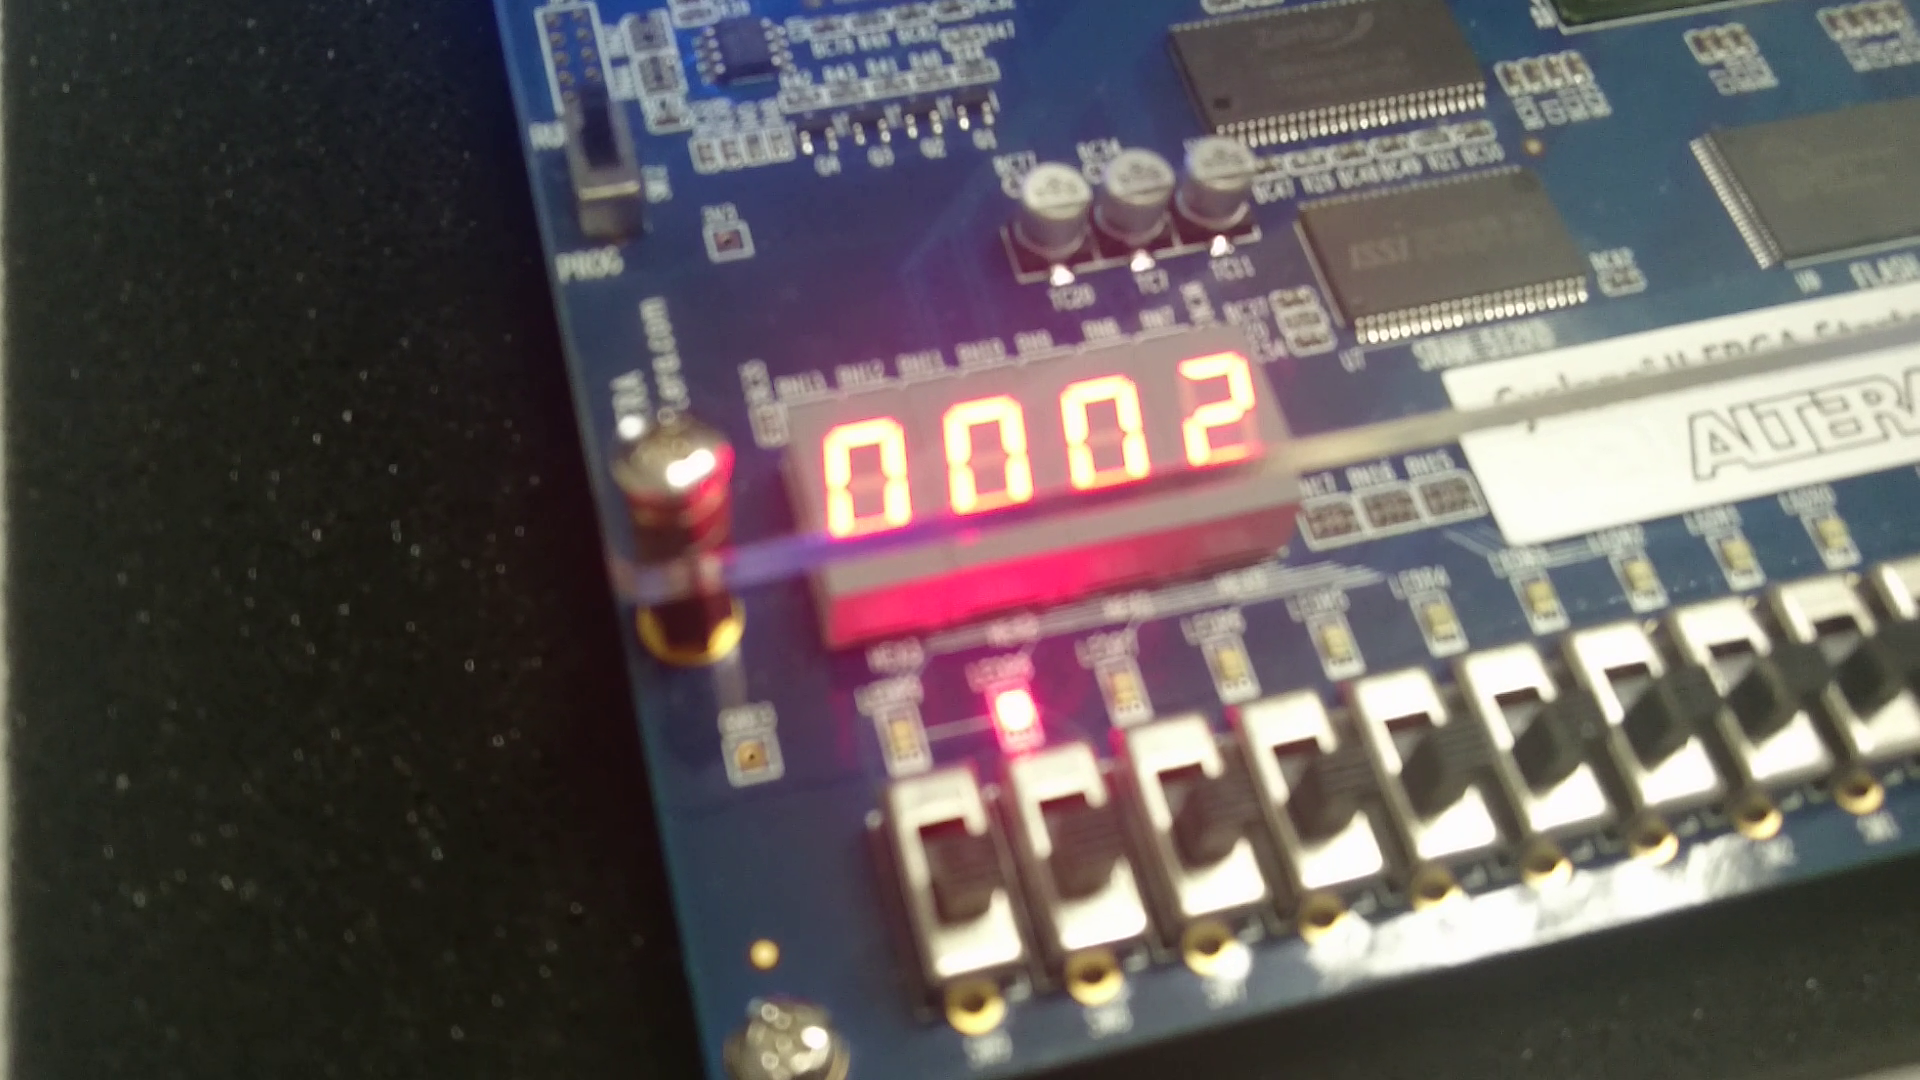
\includegraphics[width=8cm,bb=0 0 1920 1080]{1+1.png}
  \end{center}
  \caption{"1+1="}
 \end{minipage}
 \begin{minipage}{0.5\hsize}
  \begin{center}
   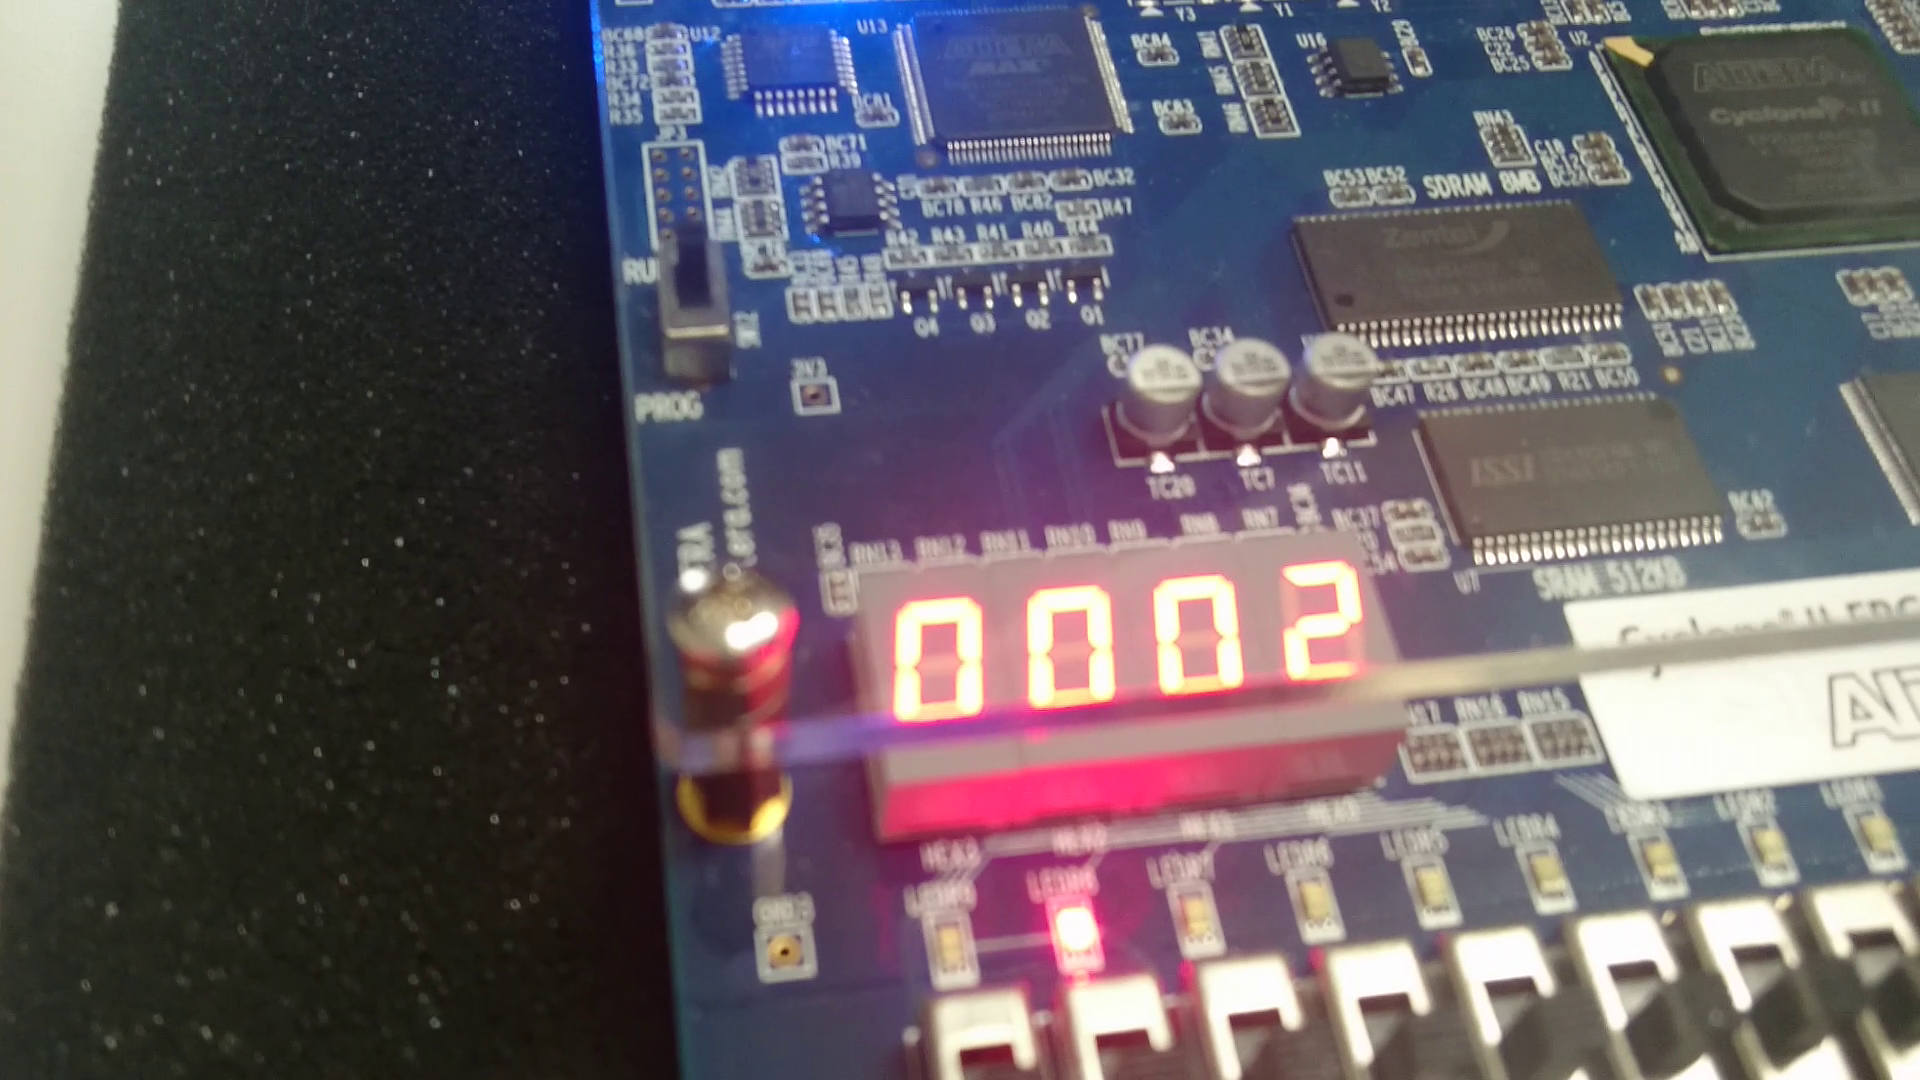
\includegraphics[width=8cm,bb=0 0 1920 1080]{3-1.png}
  \end{center}
  \caption{"3-1="}
 \end{minipage}
\end{figure}

\begin{figure}[htbp]
 \begin{minipage}{0.5\hsize}
  \begin{center}
  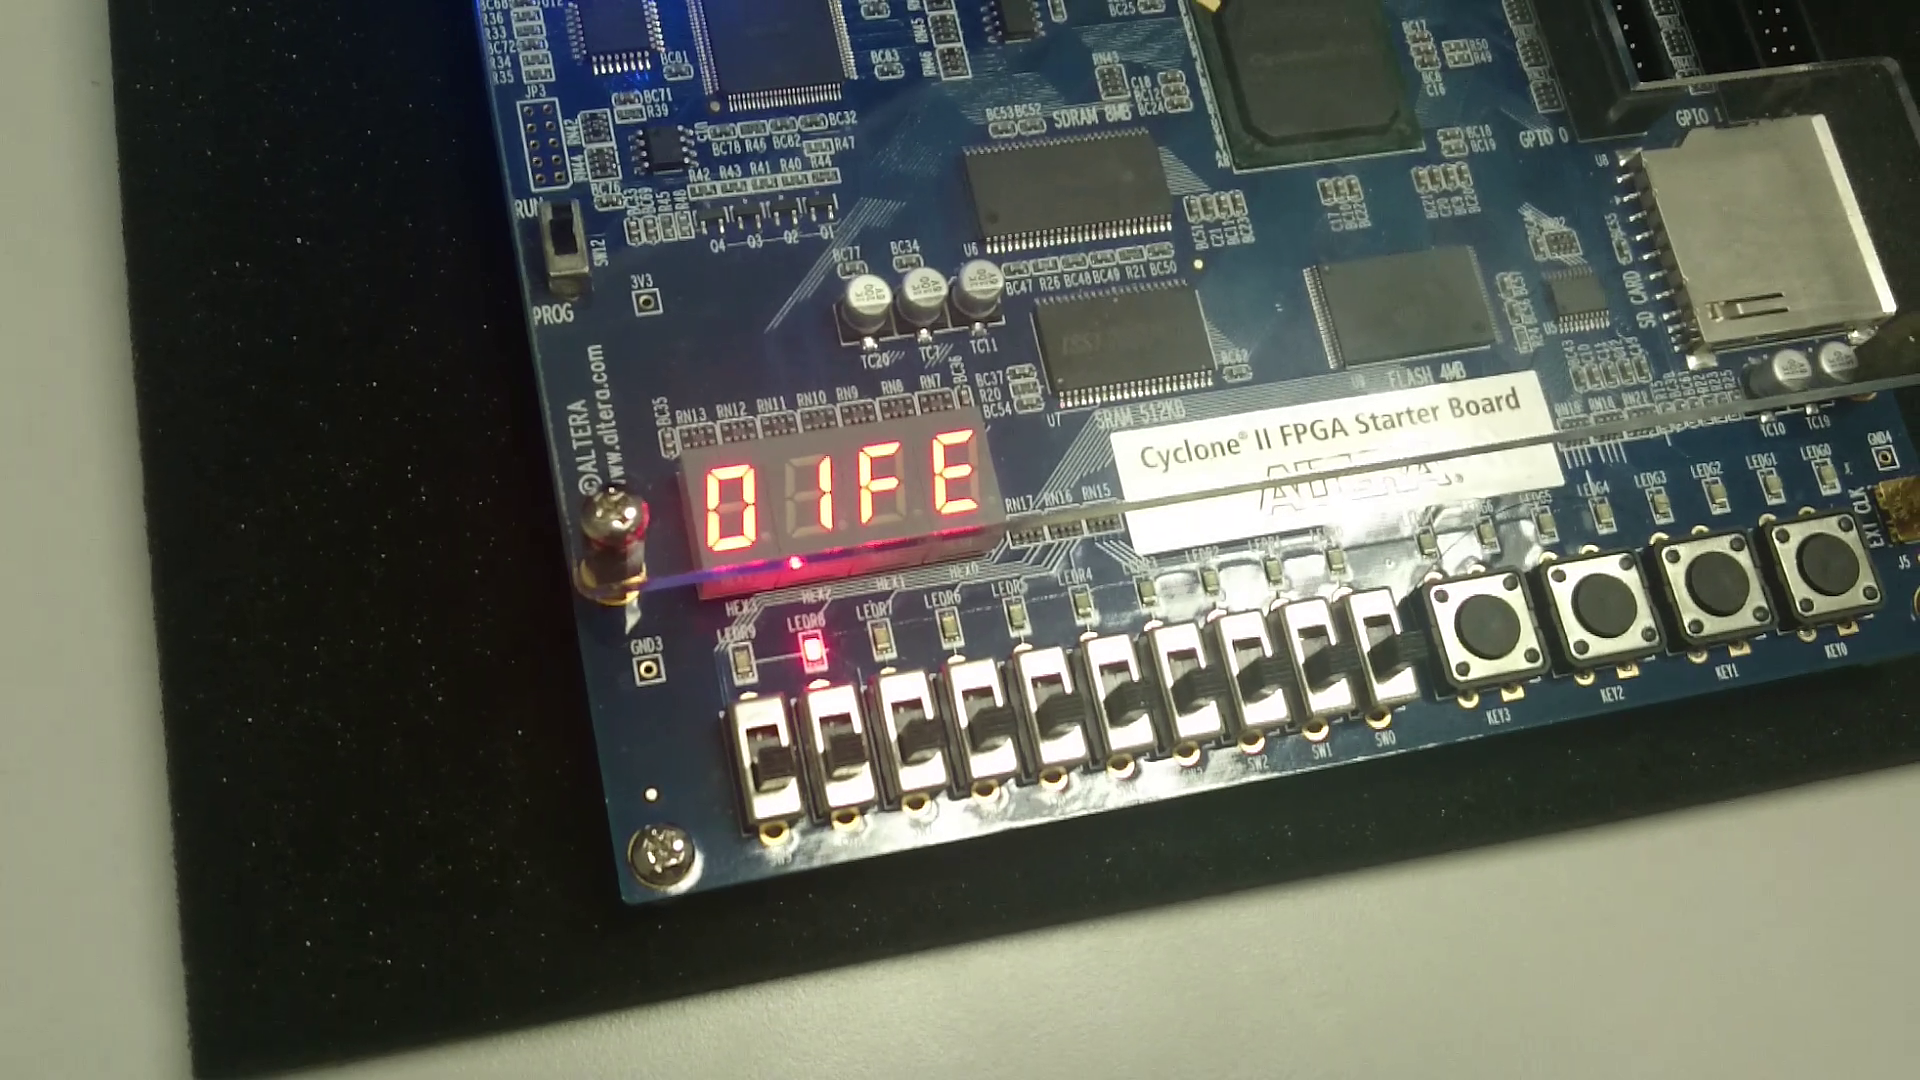
\includegraphics[width=8cm,bb=0 0 1920 1080]{FF+FF.png}
  \end{center}
  \caption{"FF+FF="}
 \end{minipage}
 \begin{minipage}{0.5\hsize}
  \begin{center}
   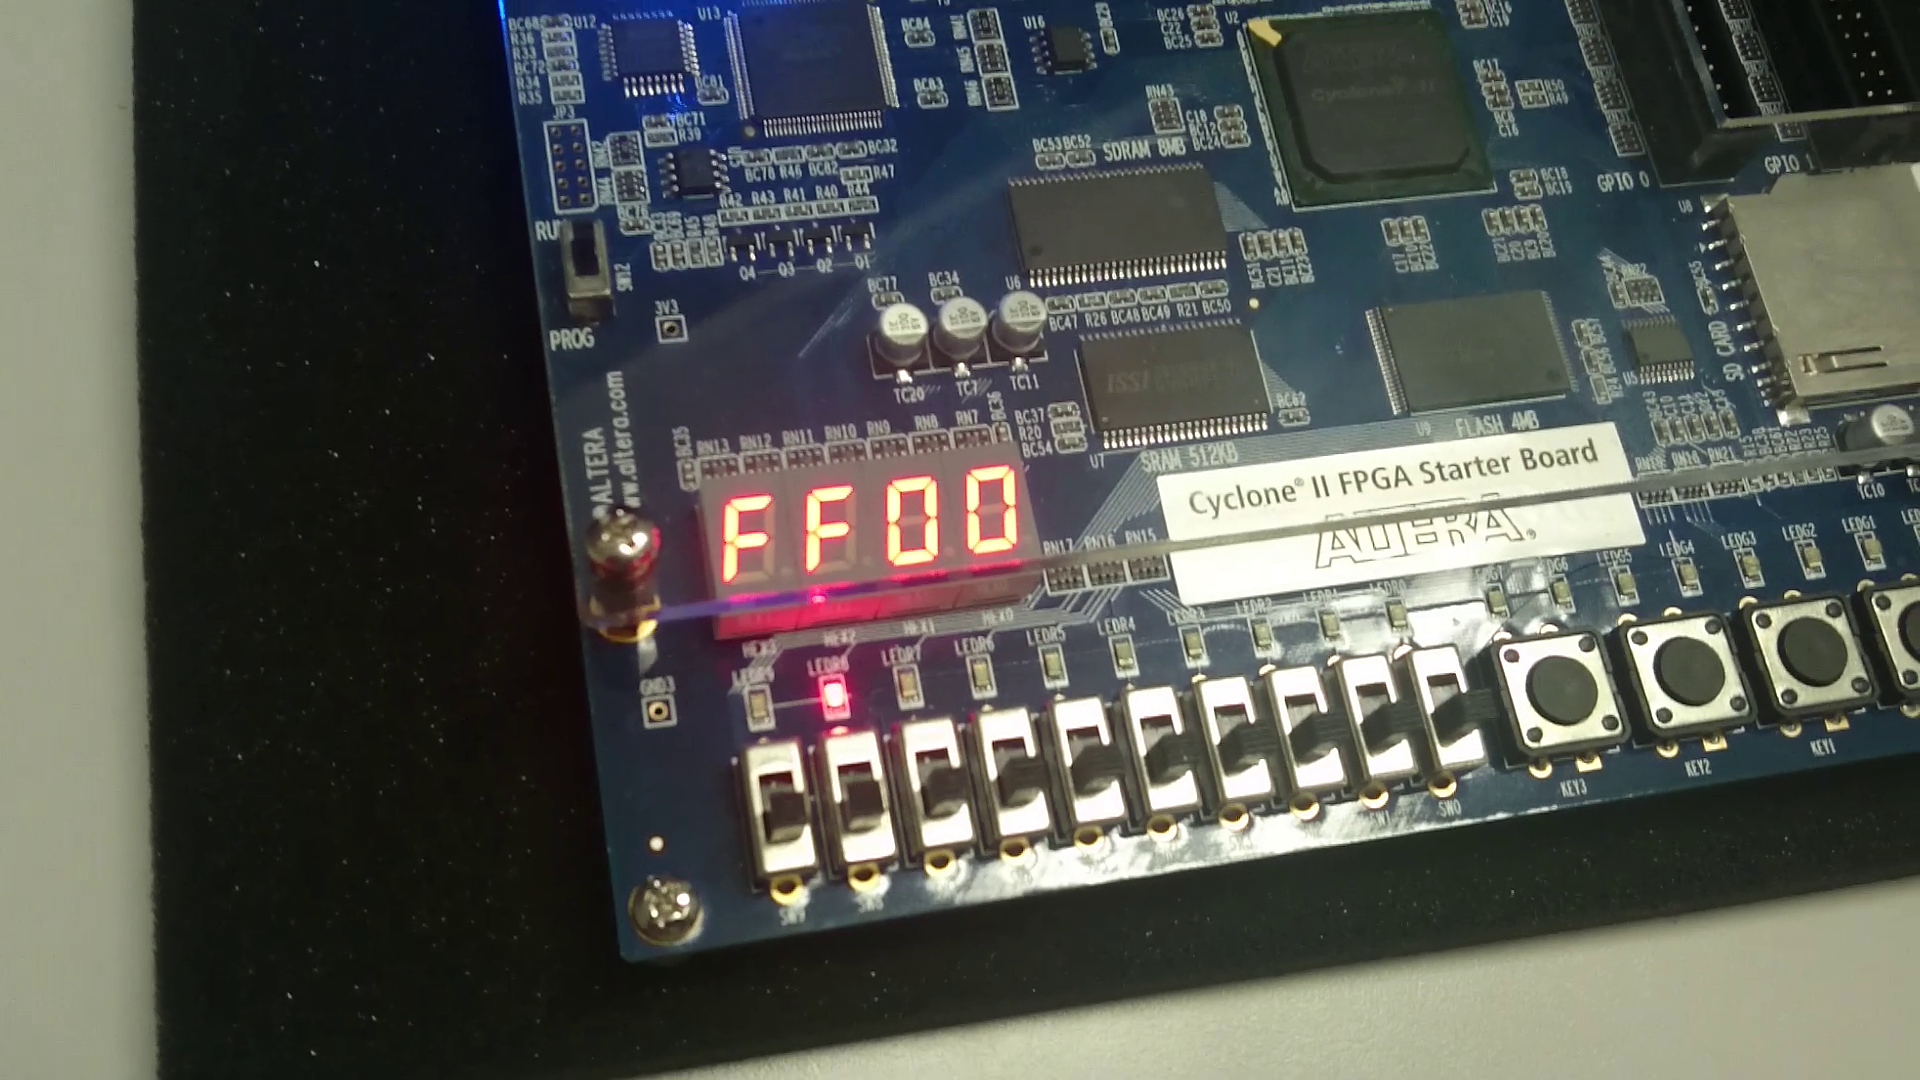
\includegraphics[width=8cm,bb=0 0 1920 1080]{FFFF-FF.png}
  \end{center}
  \caption{"FFFF-FF="}
 \end{minipage}
\end{figure}

\subsubsection*{プログラムの変更箇所}
Verilogコードで変更したファイルは、cpu\_ex3.vとfpga\_ex3.vである。
オペコードはF004,F002,F001が余っていたため、SEG命令はF004に充てることとした。
命令フェッチサイクルについてはその他の入出力命令を参考にし、4サイクル目でsegレジスタにACの値を転送することとした。

以下にプログラムの変更箇所付近のみ抜粋する。

\begin{lstlisting}[caption=cpu\_ex3.v]
module cpu_ex3 (clk, com_ctl, com_addr,
            fgi_bsy, fgi, inpr_in, /// input ports
            fgo_bsy, fgo, outr,    /// output ports
            ien, imsk, iot,
            s, r, e, bus_data, mem_data, dr, ac,
            ir, ar, pc, sc, sc_clr, seg);
    ...
    output        seg;
    ...
    wire   [15:0] seg_nxt;
    ...
    reg_dff     #16 SEG  (clk, ~com_stop, seg_nxt & {16{~com_rst}} , seg);  /// reset value = 0x0000
    ...
/// SEG :   pt & ir[2]  : seg <- ac
    ...
    assign seg_nxt = (pt & ir[2]) ? ac : seg;       /// SEG : seg <- ac
    ...
\end{lstlisting}

\begin{lstlisting}[caption=fpga\_ex3.v]
    ...
    wire    [15:0]  bus, mem, dr, ac, ir, seg;
    ...
    wire [15:0] seg_out = (SW[7:6] == 2'b11) ? {4'b0, com_addr} : seg;

    seg7_enc SEG7_E0 (seg_out[15:12],HEX3);
    seg7_enc SEG7_E1 (seg_out[11:8], HEX2);
    seg7_enc SEG7_E2 (seg_out[7:4],  HEX1);
    seg7_enc SEG7_E3 (seg_out[3:0],  HEX0);
    ...
    cpu_ex3 CPU_EX3 (clk, cpu_state, com_addr,
            fgi_bsy, fgi, inpr, /// input port
            fgo_bsy, fgo, outr, /// output port
            ien, imsk, iot,
            s, r, e, bus, mem, dr, ac, ir, ar, pc, sc, sc_clr, seg);
    ...
\end{lstlisting}

\subsubsection*{感想}
もともと7セグメント表示の雛形ができあがっていたため、流すべき情報を流すだけで動いたので楽な課題だった。
Verilogコードも初めて触れたため恐る恐る書いていたが、思ったよりも思い通りの挙動をしており書きやすかった。
掛け算命令などもVerilogコード上で実装しようとも考えたが、ループ処理を含むため他の命令に比べVerilogコードが複雑になってしまうと考え、時間がなかったことも加味して今回は断念した。
次の自由課題で挑戦してみたい。

\end{document}
